\chapter{Results}\label{chap:results}
This chapter presents the outcomes of the predictive modeling pipeline. It begins by detailing the results of the extensive model benchmarking process, leading to the selection and final evaluation of the primary classification model. Subsequently, it presents the performance and interpretation of the time-to-event models. All results were generated from the held-out test set, following the strict, leakage-aware methodology established in the preceding chapters.

\section{Supervised Mortality Prediction}
The primary objective of this thesis was the development of a binary classifier for in-hospital mortality. This was pursued through a two-stage process: benchmarking of various algorithms, followed by an in-depth evaluation of the final selected model.

\subsection{Model Benchmarking and Selection}
A wide range of classification algorithms was systematically evaluated to identify the most suitable candidate for the clinical task. The benchmark included traditional statistical models (Logistic Regression, LDA), regularized linear models (Ridge, Lasso, ElasticNet), and more complex, non-linear ensembles (Random Forest, XGBoost, LightGBM, DNN++). To address the inherent class imbalance in the dataset, two primary strategies were compared: intrinsic class weighting and various oversampling techniques (e.g., SMOTE, BorderlineSMOTE).

The results of this benchmark are summarized in Table~\ref{tab:ml_benchmark}. A clear trend emerged: tree-based ensembles consistently outperformed linear models in terms of discrimination, as measured by the ROC-AUC. The \textbf{LightGBM model trained with class weights} was identified as the top-performing model, achieving the highest ROC-AUC of 0.749 in the initial validation. While oversampling methods tended to produce higher F1-scores, this was often at the expense of precision and did not yield a superior ROC-AUC. Given that the primary goal was to accurately discriminate high-risk from low-risk patients across all decision thresholds, ROC-AUC was prioritized, and the LightGBM model was selected for the final stage of tuning, calibration, and evaluation.

\begin{table}[htb!]
    \centering
    \caption{Best performance by algorithm type from the benchmarking experiments, sorted by ROC-AUC.}
    \label{tab:ml_benchmark}
    \begin{tabular}{lrr}
        \toprule
        \textbf{Model Algorithm} & \textbf{ROC-AUC} & \textbf{F1-Score} \\
        \midrule
        LightGBM & 0.7492 & 0.4129 \\
        XGBoost & 0.7444 & 0.4527 \\
        Logistic Regression & 0.7382 & 0.5227 \\
        Linear Discriminant Analysis (LDA) & 0.7364 & 0.3756 \\
        ElasticNet & 0.7363 & 0.5185 \\
        Ridge & 0.7349 & 0.5174 \\
        Deep Neural Network (DNN++) & 0.7347 & 0.4471 \\
        Lasso & 0.7331 & 0.5244 \\
        Random Forest & 0.7137 & 0.3468 \\
        \bottomrule
    \end{tabular}
\end{table}

\subsection{Final Model Performance on the Test Set}
The selected LightGBM model was subjected to a final evaluation pipeline. After hyperparameter tuning with Optuna, the model's raw outputs were calibrated using isotonic regression on a validation split of the training data. The optimal classification threshold was determined to be 0.2704 by maximizing Youden's J statistic on this same validation set.

The final, calibrated model was then applied to the unseen held-out test set. The model achieved a ROC-AUC of 0.749, which was taken as evidence of strong and generalizable discriminative ability. The complete performance metrics are detailed in Table~\ref{tab:final_performance}. The confusion matrix (Figure~\ref{fig:confusion_matrix_roc}a) provides a clear picture of the model's performance at the chosen clinical threshold: it correctly identified 368 of the 537 patients who died (a recall of 0.685) while maintaining a precision of 0.422. The ROC curve (Figure~\ref{fig:confusion_matrix_roc}b) further illustrates the model's consistent performance across the full range of decision thresholds.

\begin{table}[htb!]
    \centering
    \caption{Performance of the final calibrated LightGBM model on the held-out test set.}
    \label{tab:final_performance}
    \begin{tabular}{lr}
        \toprule
        \textbf{Metric} & \textbf{Value} \\
        \midrule
        ROC-AUC & 0.7488 \\
        Accuracy & 0.6648 \\
        Precision & 0.4220 \\
        Recall (Sensitivity) & 0.6853 \\
        F1-Score & 0.5224 \\
        \bottomrule
    \end{tabular}
\end{table}

\begin{figure}[htb!]
    \centering
    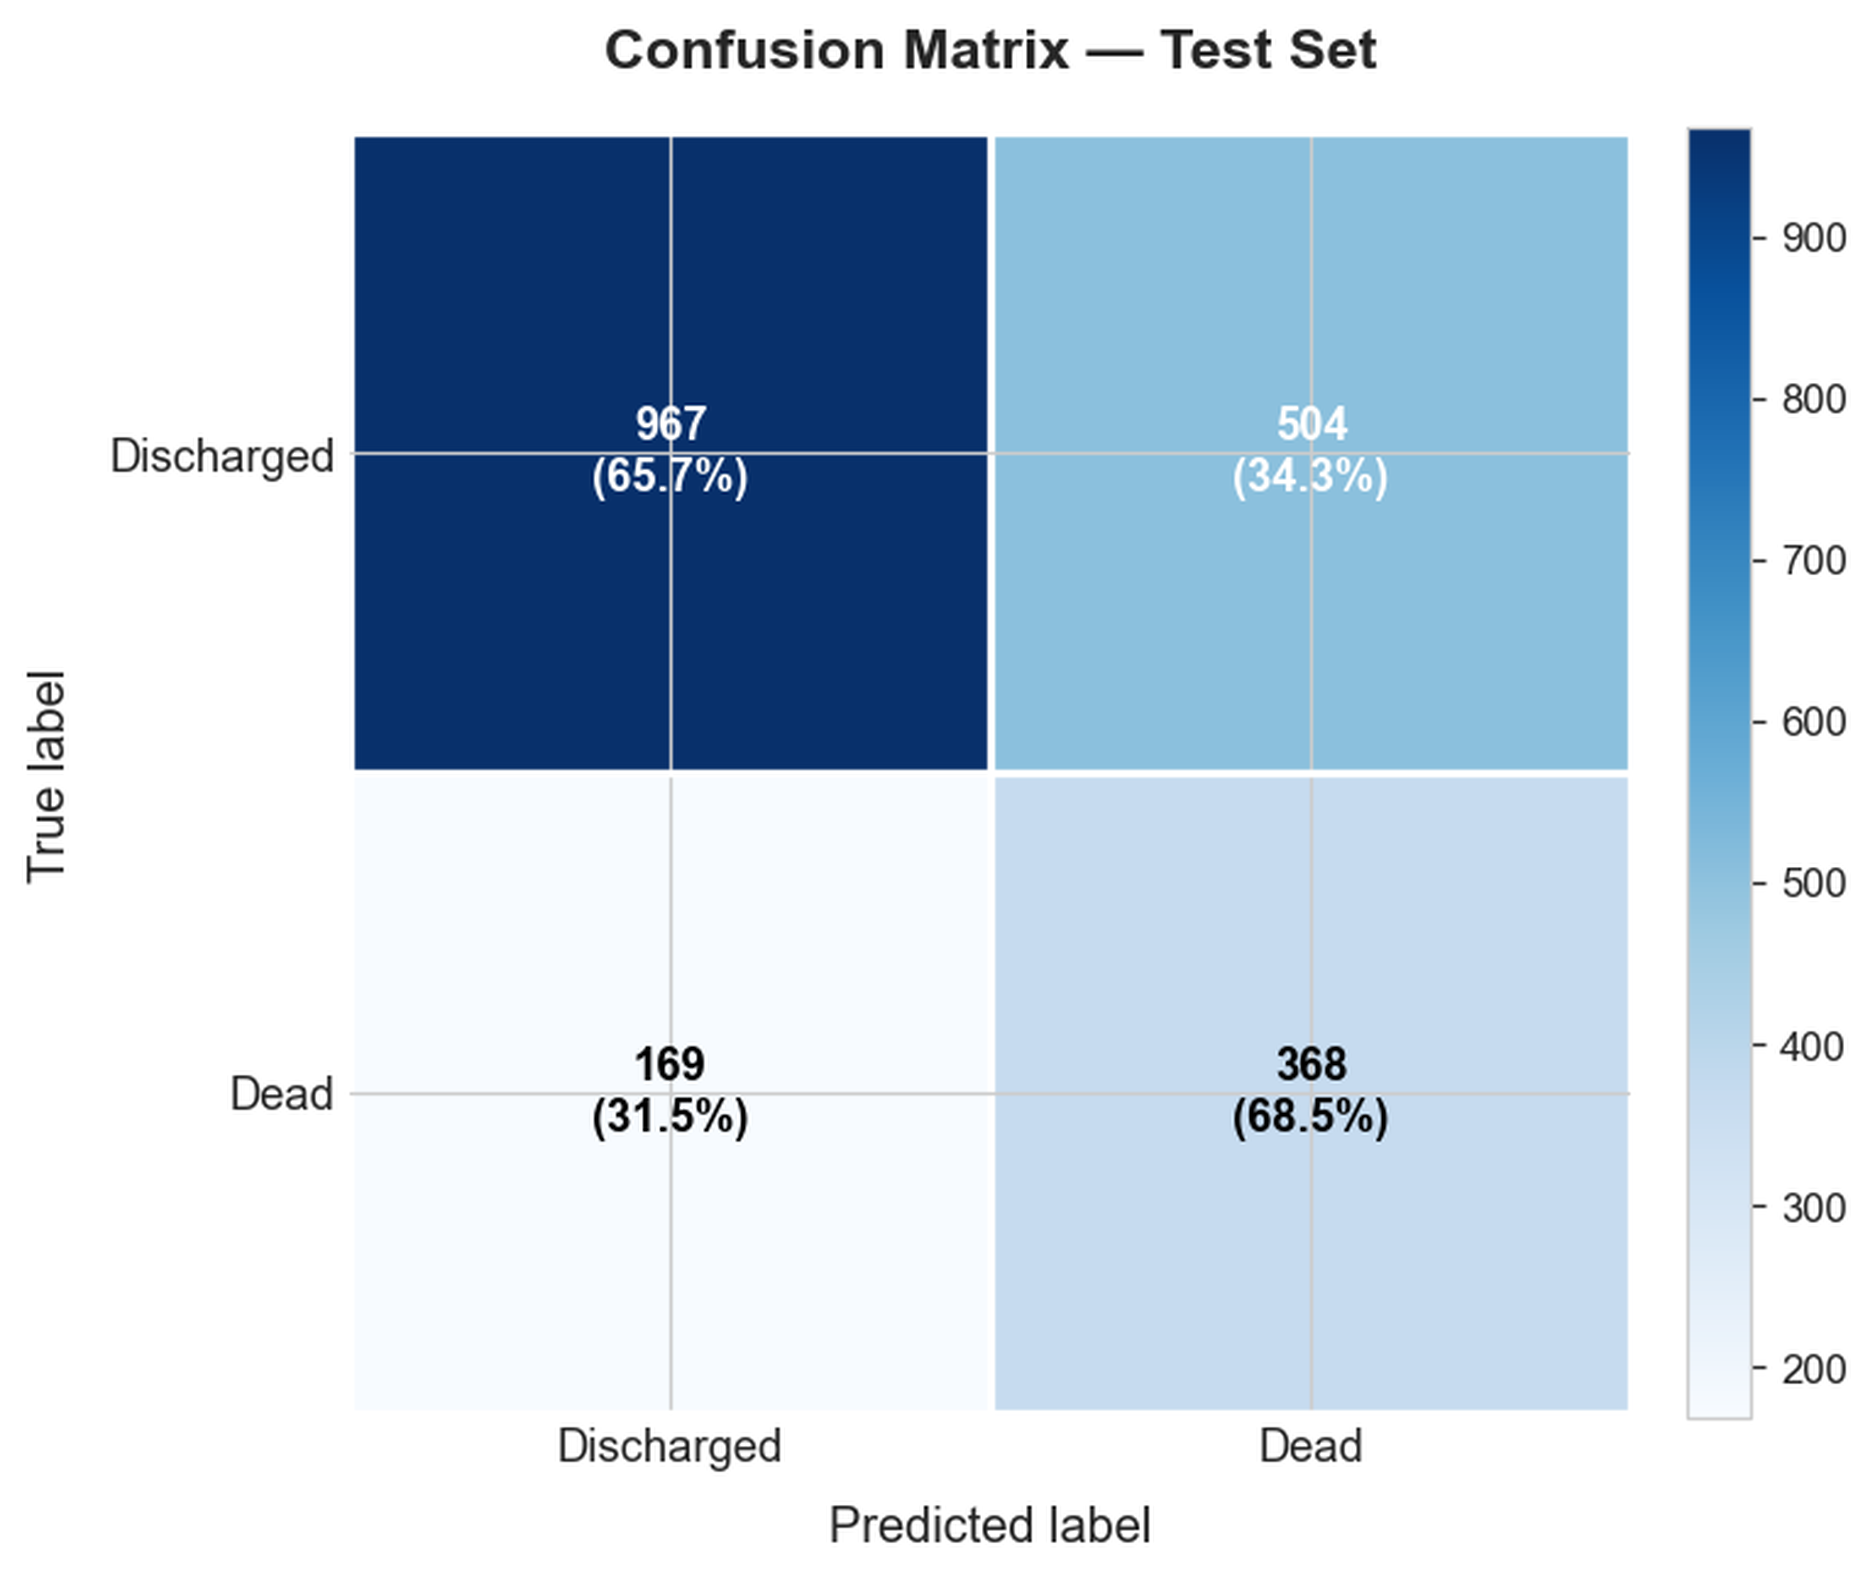
\includegraphics[width=0.5\textwidth]{ml_images/confusion_matrix.png}\hfill
    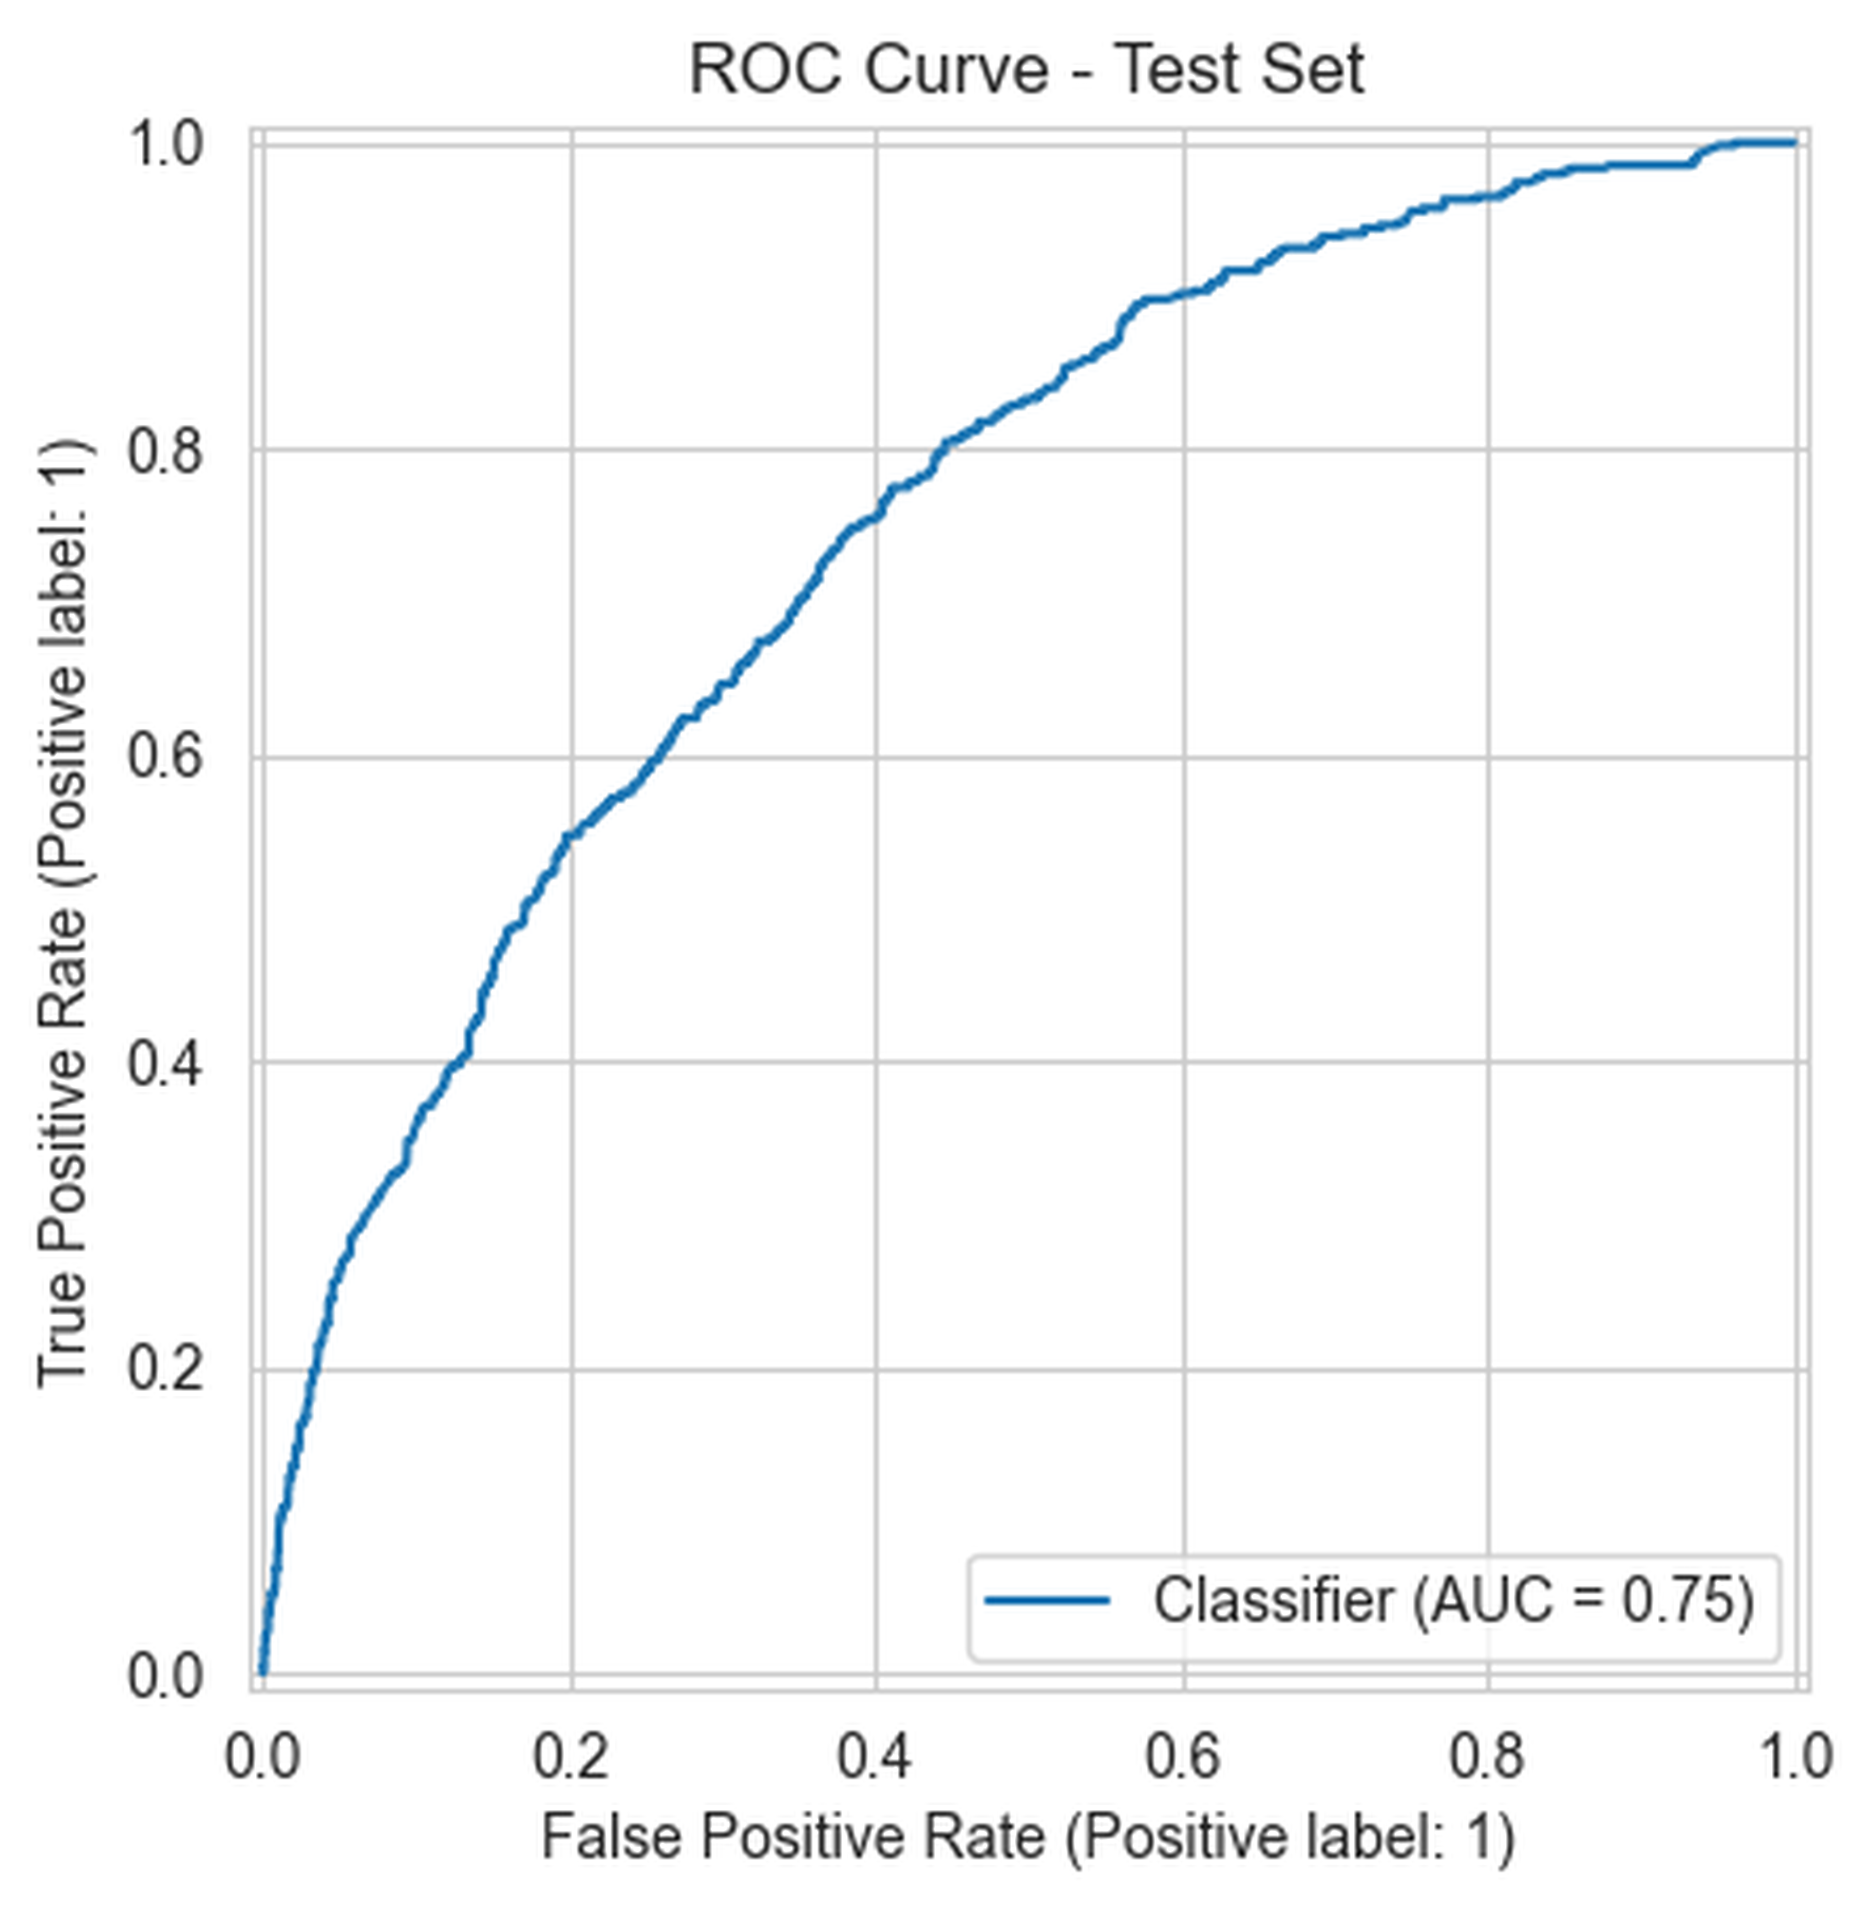
\includegraphics[width=0.5\textwidth]{ml_images/roc_curve.png}
    \caption{(\textbf{a}) Confusion matrix of the final model on the test set at the optimal threshold (0.2704). (\textbf{b}) ROC curve for the final model on the test set, showing an AUC of 0.75.}
    \label{fig:confusion_matrix_roc}
\end{figure}

\subsection{Model Interpretability with SHAP}
To ensure the model's clinical relevance and transparency, its predictions were interpreted using SHAP. The beeswarm plot in Figure~\ref{fig:shap_beeswarm} provides a global summary of the features driving the model's output. This analysis suggests that the model's logic aligns with established clinical knowledge.

The most influential feature was the \texttt{sofa\_total\_24hr} score, a global measure of organ dysfunction. Other key predictors of mortality included markers of hematological dysfunction (\texttt{rdw\_median\_pct}), overall illness severity (\texttt{apache\_iii\_score}), advanced age, and renal failure (\texttt{bun\_median}). Conversely, higher urine output (\texttt{urine\_output\_total\_24hr}), a sign of preserved kidney function, was a strong predictor of survival. This concordance between the model's learned patterns and clinical pathophysiology has been interpreted as evidence supporting its validity.

\begin{figure}[htb!]
    \centering
    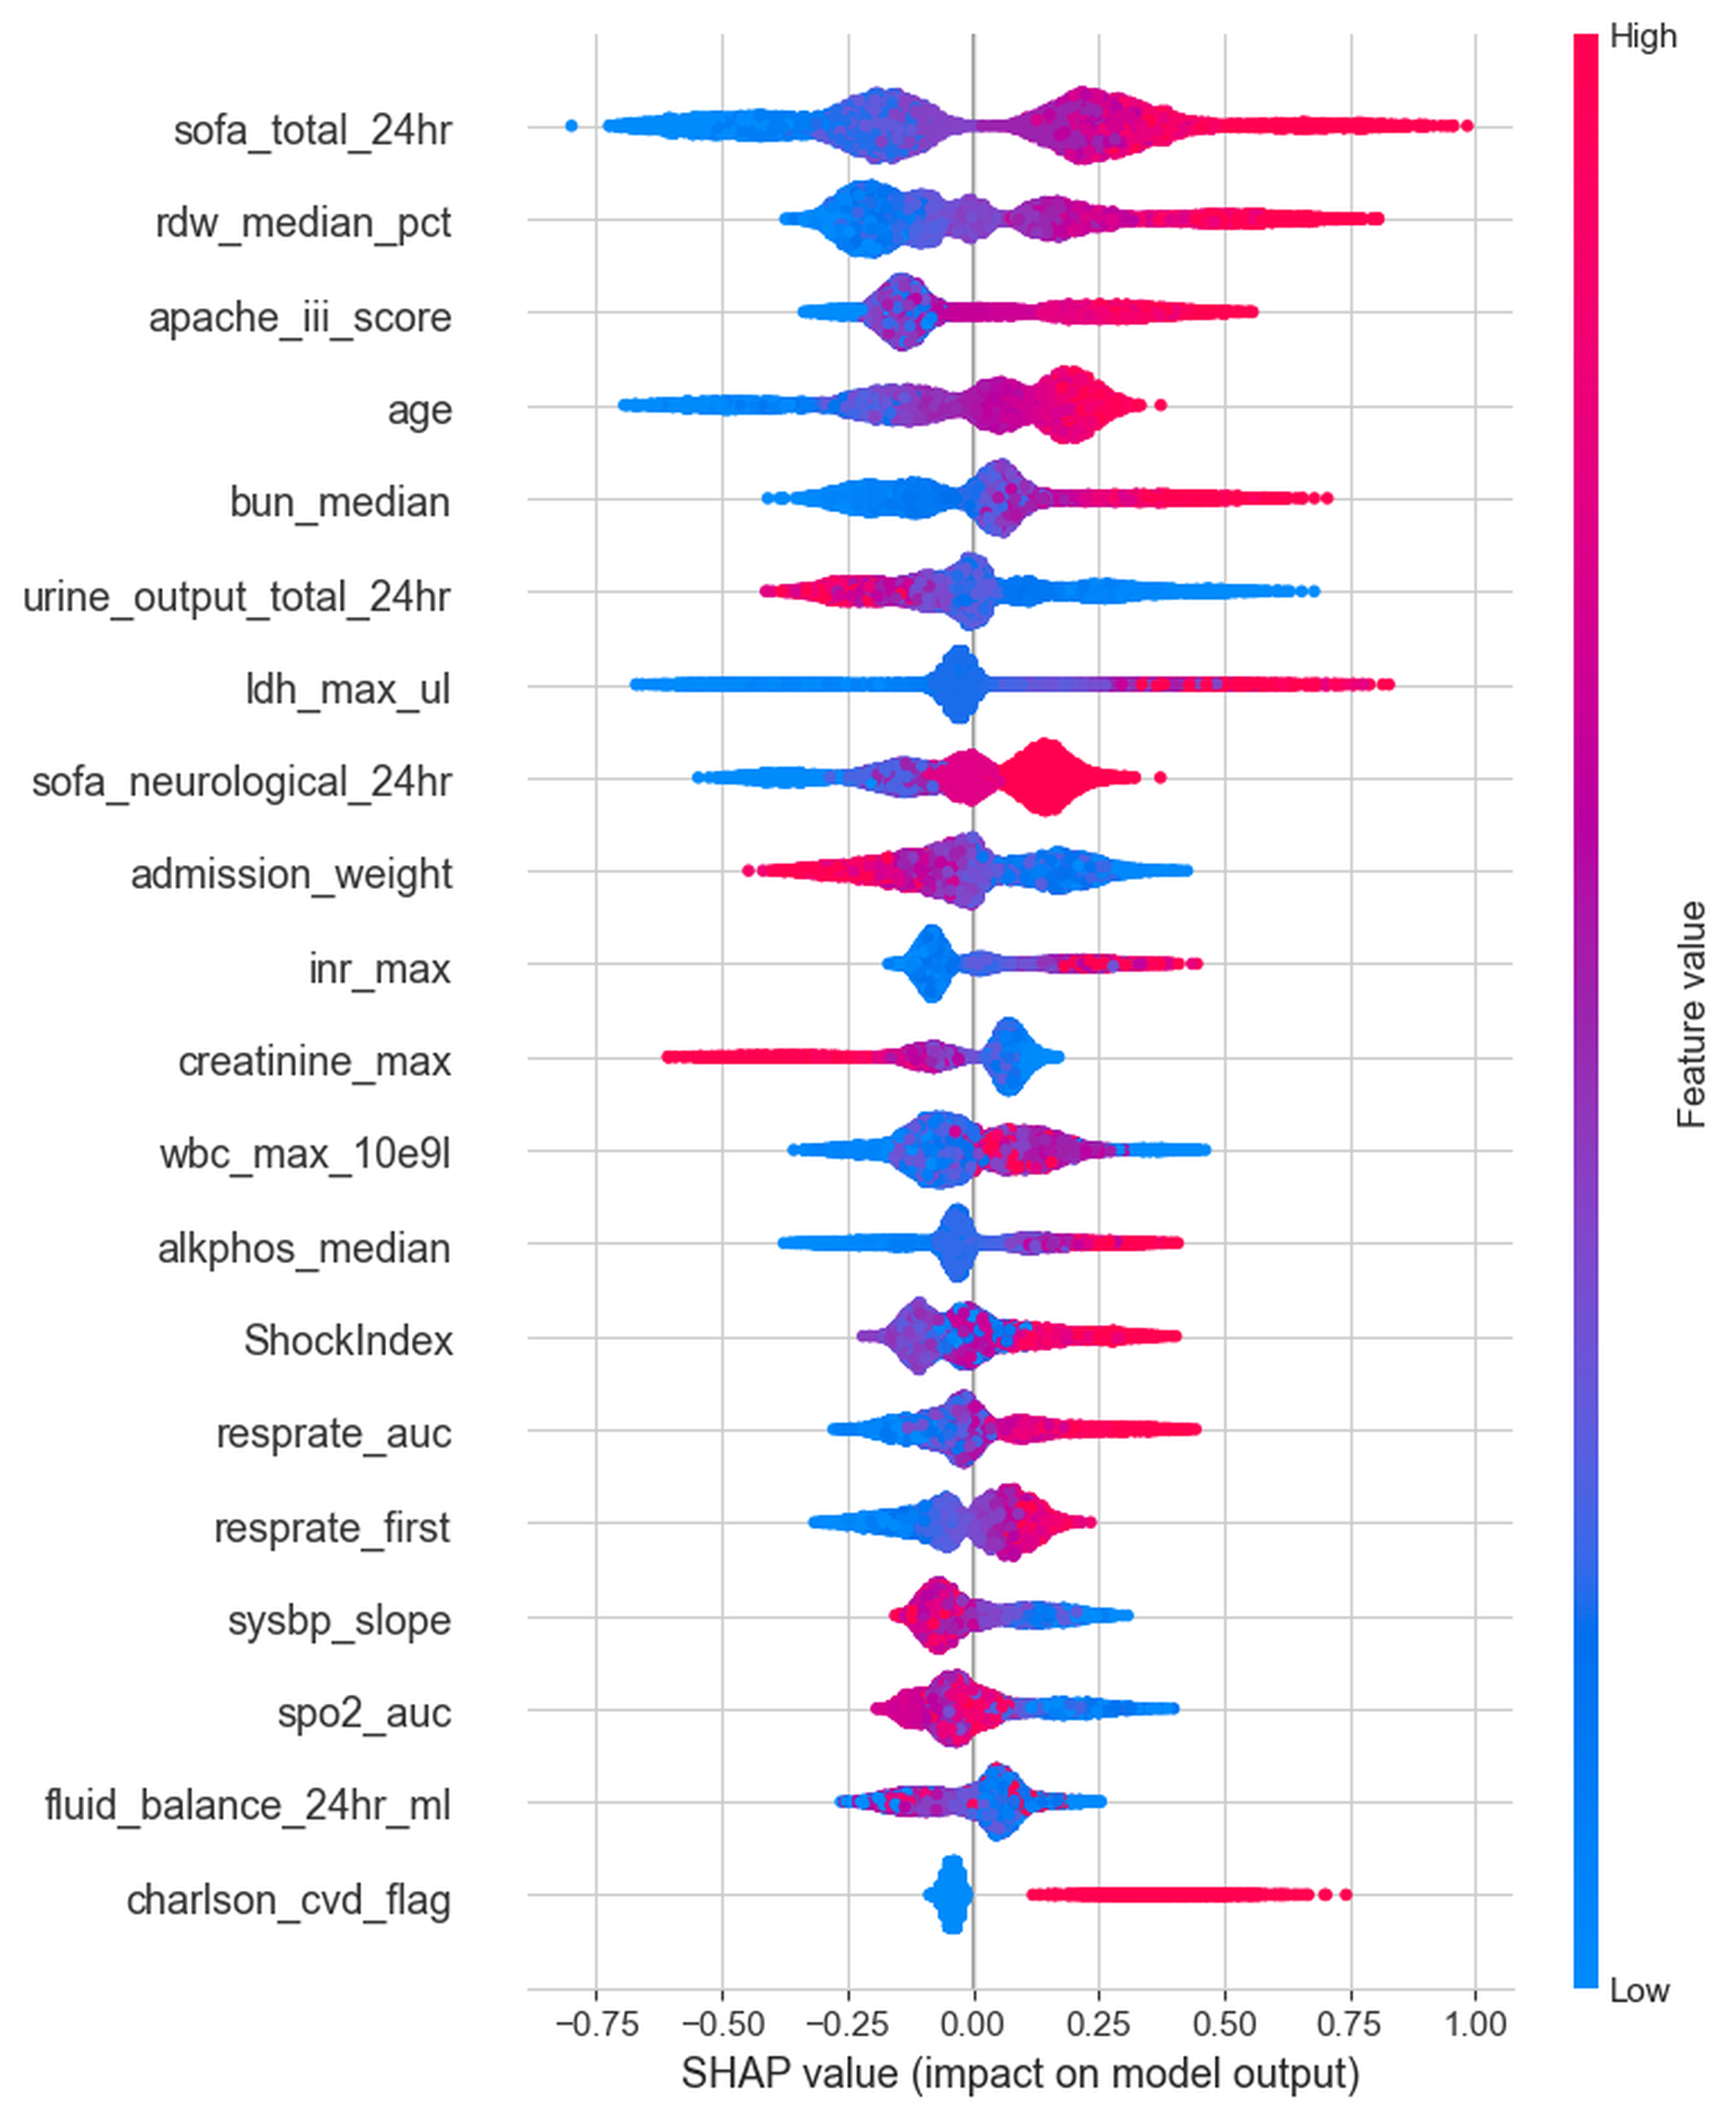
\includegraphics[width=0.8\textwidth]{ml_images/shap_beeswarm.png}
    \caption{SHAP beeswarm summary plot for the top 20 features. Each dot represents a patient. The feature's value is indicated by color (red=high, blue=low), and its impact on the mortality prediction is shown on the x-axis.}
    \label{fig:shap_beeswarm}
\end{figure}

\subsection{Why LightGBM Outperforms Other Model Classes}
The selection of LightGBM as the final model was not arbitrary but was driven by its consistent superiority in the benchmark (Table~\ref{tab:ml_benchmark}). Several properties of the algorithm have been identified as contributing to this advantage in the context of SA--AKI mortality prediction.

LightGBM employs a leaf-wise tree growth strategy rather than the level-wise approach adopted by traditional gradient boosting implementations. This design concentrates splitting effort on the leaves that yield the largest reduction in loss, a property that has been found to be particularly effective when the feature space contains a mixture of continuous biomarkers with skewed distributions and sparse binary indicators such as comorbidity flags and missingness indicators. In addition, LightGBM natively captures the interaction structure that characterizes clinical data. SA--AKI mortality is not driven by any single variable in isolation but rather by the joint configuration of organ dysfunction scores, hemodynamic instability, and metabolic derangement. Tree ensembles represent these higher-order interactions without requiring explicit feature engineering, whereas linear models (Logistic Regression, Ridge, Lasso, ElasticNet) are constrained to additive main effects unless interactions are manually specified. This distinction is reflected in the benchmark: the best-performing linear model (Logistic Regression, AUROC 0.738) trailed LightGBM (AUROC 0.749) by a margin that, while modest in absolute terms, was observed to be consistent across cross-validation folds and to correspond to meaningful reclassification of patients near the decision boundary.

The handling of class imbalance further differentiated LightGBM from alternative approaches. The built-in \texttt{class\_weight='balanced'} mechanism, which reweights the loss function inversely proportional to class frequency, was found to be more effective than synthetic oversampling (SMOTE, ADASYN) for this dataset. Oversampling methods tended to inflate recall at the cost of precision without improving overall discrimination, a pattern consistent with the known risks of synthesizing examples in overlapped regions of the feature space \citep{Blagus_2013,Saez_2015}. The Optuna-based hyperparameter search explored a richer space than grid search, encompassing regularization parameters (\texttt{reg\_alpha}, \texttt{reg\_lambda}), tree depth, minimum child samples, and feature and bagging fractions, which collectively controlled overfitting and contributed to improved generalization on the held-out test set.

\subsection{Evidence for Trustworthiness and Clinical Credibility}
A clinician evaluating a risk score requires more than a single discrimination metric; the credibility of the model must be established through multiple complementary lines of evidence. The trustworthiness of the predictions presented here has been assessed along five dimensions.

The first dimension concerns methodological integrity. The AUROC of 0.749 was obtained under conditions specifically designed to prevent optimistic bias: all preprocessing was fitted exclusively on training data, no post-T24 information entered the feature set, the test set was used exactly once for final evaluation, and no feature selection or imputation step was permitted access to test-set outcomes. In contrast, studies reporting AUROC values of 0.79--0.88 for SA--AKI mortality have been found to include length of stay as a predictor \citep{Chen_2025}, to perform feature selection on the full dataset \citep{Li_2023_SciRep}, or to employ whole-stay aggregation windows that embed future information. When these methodological advantages are removed, the achievable discrimination for a genuine early warning system would be expected to be lower, and the result obtained here is consistent with that expectation.

The second dimension relates to calibration. The predicted probabilities were explicitly calibrated using isotonic regression on a validation split, ensuring that when the model assigns a 30\% risk of death, approximately 30\% of patients in that probability bin were observed to have died. Calibration is essential for clinical utility because treatment decisions depend on the absolute magnitude of risk rather than merely on the ranking of patients. It has been noted that several prior studies did not report calibration at all \citep{Chen_2025,Li_2023_SciRep}.

The third dimension is clinical face validity, as assessed through SHAP analysis. The SHAP analysis (Figure~\ref{fig:shap_beeswarm}) confirmed that the top predictors identified by the model (SOFA score, RDW, APACHE~III, age, BUN, and urine output) are established clinical risk factors for ICU mortality. A model whose predictions are driven by clinically interpretable signals has been considered more likely to generalize than one that exploits dataset-specific artifacts.

The fourth dimension involves decision-curve analysis. The survival models were shown to demonstrate positive net benefit over the ``treat all'' and ``treat none'' strategies across a clinically relevant range of risk thresholds (8--30\%), providing direct evidence that the use of the model to inform decisions would be expected to improve outcomes compared with default strategies (Figure~\ref{fig:deepsurv_dca}).

The fifth dimension is the concordance observed across fundamentally different model families. The consistency of results across LightGBM (AUROC 0.749), CoxPH (C-index 0.693), and DeepSurv (C-index 0.688) provides a form of triangulation. If the predictive signal were spurious or driven by leakage, it would be unlikely to manifest consistently across a gradient-boosted classifier, a semi-parametric survival model, and a neural survival network.

\subsection{Comparison with Prior Work and the Case for a Realistic Benchmark}
Recent studies on SA--AKI mortality using MIMIC--IV have reported ROC--AUC values ranging from 0.79 to 0.88 \citep{Chen_2025,Li_2023_SciRep,Qu_2024}. However, as discussed in Chapter~\ref{chap:litreview}, many of these results are likely to represent overestimations arising from methodological shortcomings: information leakage through whole-stay data aggregation, inclusion of length of stay as a predictor, global fitting of preprocessing steps, and the absence of calibration. The key methodological differences are summarized in Table~\ref{tab:comparison_prior}.

\begin{table}[htb!]
    \centering
    \caption{Methodological comparison with representative prior SA--AKI mortality studies.}
    \label{tab:comparison_prior}
    \small
    \begin{tabular}{lcccc}
        \toprule
        \textbf{Criterion} & \textbf{This work} & \textbf{Chen (2025)} & \textbf{Li (2023)} & \textbf{Hu (2021)} \\
        \midrule
        Feature window & T0--T24 & Unspecified & T0--T24 & Whole-stay \\
        LOS as predictor & No & Yes & No & No \\
        Train-only preprocessing & Yes & No & No & No \\
        Missingness indicators & Yes & No & No & No \\
        Explicit calibration & Yes & No & No & No \\
        Separate validation set & Yes & No & No & No \\
        Reported AUROC & 0.749 & 0.878 & 0.794 & --- \\
        Reported C-index & 0.69 & --- & --- & 0.72 \\
        \bottomrule
    \end{tabular}
\end{table}

The AUROC of 0.749 should therefore be interpreted not as an inferior result but as a more realistic and credible estimate of what is achievable for a genuine early warning system that relies exclusively on information available at the bedside within 24 hours of ICU admission. This work has been positioned as a methodologically sound benchmark against which future studies may be compared on equal footing.

\subsection{Limitations: External Validation and Dataset Scope}\label{sec:external-validation}
A key limitation of this work, shared with the majority of SA--AKI prediction studies, is the absence of external validation on an independent dataset. The model was developed and evaluated exclusively on MIMIC--IV, which reflects the patient population, clinical practices, and documentation patterns of a single tertiary-care center (Beth Israel Deaconess Medical Center, Boston). Performance drift across hospitals has been documented in the ICU prediction literature \citep{Rockenschaub_2024}, and the degree to which the model would generalize to other institutions remains an open empirical question.

The most natural candidate for external validation has been identified as the eICU Collaborative Research Database, a multi-center dataset covering over 200 hospitals across the United States. However, eICU presents several harmonization challenges that would need to be addressed: differences in laboratory item coding, variable availability (certain biomarkers may be less consistently recorded across sites), and population-level differences in case mix and care intensity. A careful external validation would require re-application of the same cohort definition (Sepsis--3 + KDIGO), re-derivation of T0--T24 features from the eICU schema, and evaluation of the frozen model without retraining. This has been identified as the immediate next step in Chapter~\ref{chap:conclusion}.

Until external validation has been completed, the model's predictions should be interpreted as internally valid risk estimates specific to the MIMIC--IV population. Recalibration on the target population would be expected to be necessary before the model could be considered for bedside decision support at any external institution. It has been noted that many prior studies have claimed broad generalizability without providing external evidence to support such claims \citep{Chen_2025}, and the explicit acknowledgment of this limitation in the present work has been intended to encourage more transparent reporting practices in the field.

\section{Time-to-Event (Survival) Analysis}
To provide a more dynamic assessment of patient risk, survival models were developed to predict the time to in-hospital death using the same T0--T24 feature set.

\subsection{Cox Proportional Hazards Model}
After feature selection and penalization tuning, the final Cox Proportional Hazards (CoxPH) model achieved a test C-index of 0.693, indicating good discriminative ability over time. The forest plot in Figure~\ref{fig:cox_forest_plot} reveals the key drivers of hazard. Comorbidities like metastatic cancer and high SOFA scores were the strongest predictors of an increased hazard of death. Of note, early interventions such as RRT and vasopressor use were associated with a reduced hazard, a finding that is likely attributable to confounding by indication, whereby the sickest patients receive the most aggressive interventions, rather than to a causal protective effect of the therapies themselves. The model's ability to effectively stratify patients into distinct risk groups was confirmed by the clear separation of Kaplan-Meier curves for its predicted risk quartiles (Figure~\ref{fig:cox_km_quartiles}, log-rank $p < 0.001$).

\begin{figure}[htb!]
    \centering
    
\includegraphics[width=0.85\textwidth]{survival_images/cox_forest_plot.png}
    \caption{Forest plot of hazard ratios for the top 20 predictors in the final CoxPH model. Values to the right of the dashed line (HR > 1) indicate an increased risk of death.}
    \label{fig:cox_forest_plot}
\end{figure}

\begin{figure}[htb!]
    \centering
    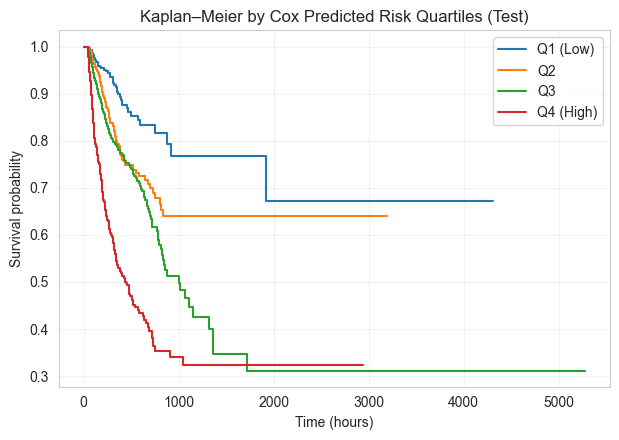
\includegraphics[width=0.8\textwidth]{survival_images/cox_km_quartiles.png}
    \caption{Kaplan-Meier survival curves for the test set, stratified by risk quartiles predicted by the CoxPH model, demonstrating effective risk stratification.}
    \label{fig:cox_km_quartiles}
\end{figure}

\subsection{DeepSurv Model}
A custom neural network-based survival model, DeepSurv, was also developed and achieved a comparable test C-index of 0.688. Like the Cox model, it demonstrated strong risk stratification (Figure~\ref{fig:deepsurv_km_tertiles}, log-rank $p < 0.001$). The clinical utility of the DeepSurv model was further interrogated through calibration and decision curve analysis (DCA). The calibration plots (Figure~\ref{fig:deepsurv_calibration}) showed good agreement between predicted and observed event probabilities at key clinical horizons, although with a slight tendency to overestimate risk in the highest-risk bins, a pattern that could be addressed in future work with more advanced calibration techniques. The DCA (Figure~\ref{fig:deepsurv_dca}) demonstrated that the use of the model to inform clinical decisions provides a net benefit over the default strategies of treating all or no patients for risk thresholds between 8\% and 30\%.

\begin{figure}[htb!]
    \centering
    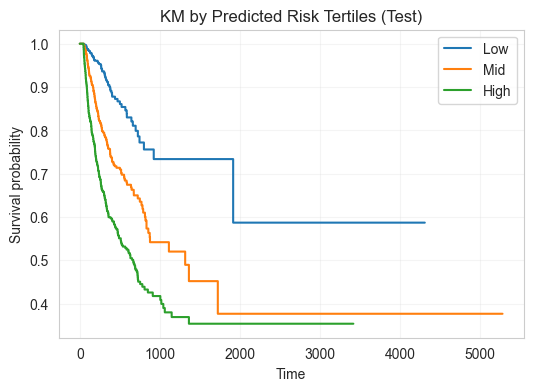
\includegraphics[width=0.7\textwidth]{survival_images/deepsurv_km_tertiles.png}
    \caption{Kaplan-Meier survival curves for the test set, stratified by risk tertiles predicted by the DeepSurv model.}
    \label{fig:deepsurv_km_tertiles}
\end{figure}

\begin{figure}[htb!]
    \centering
    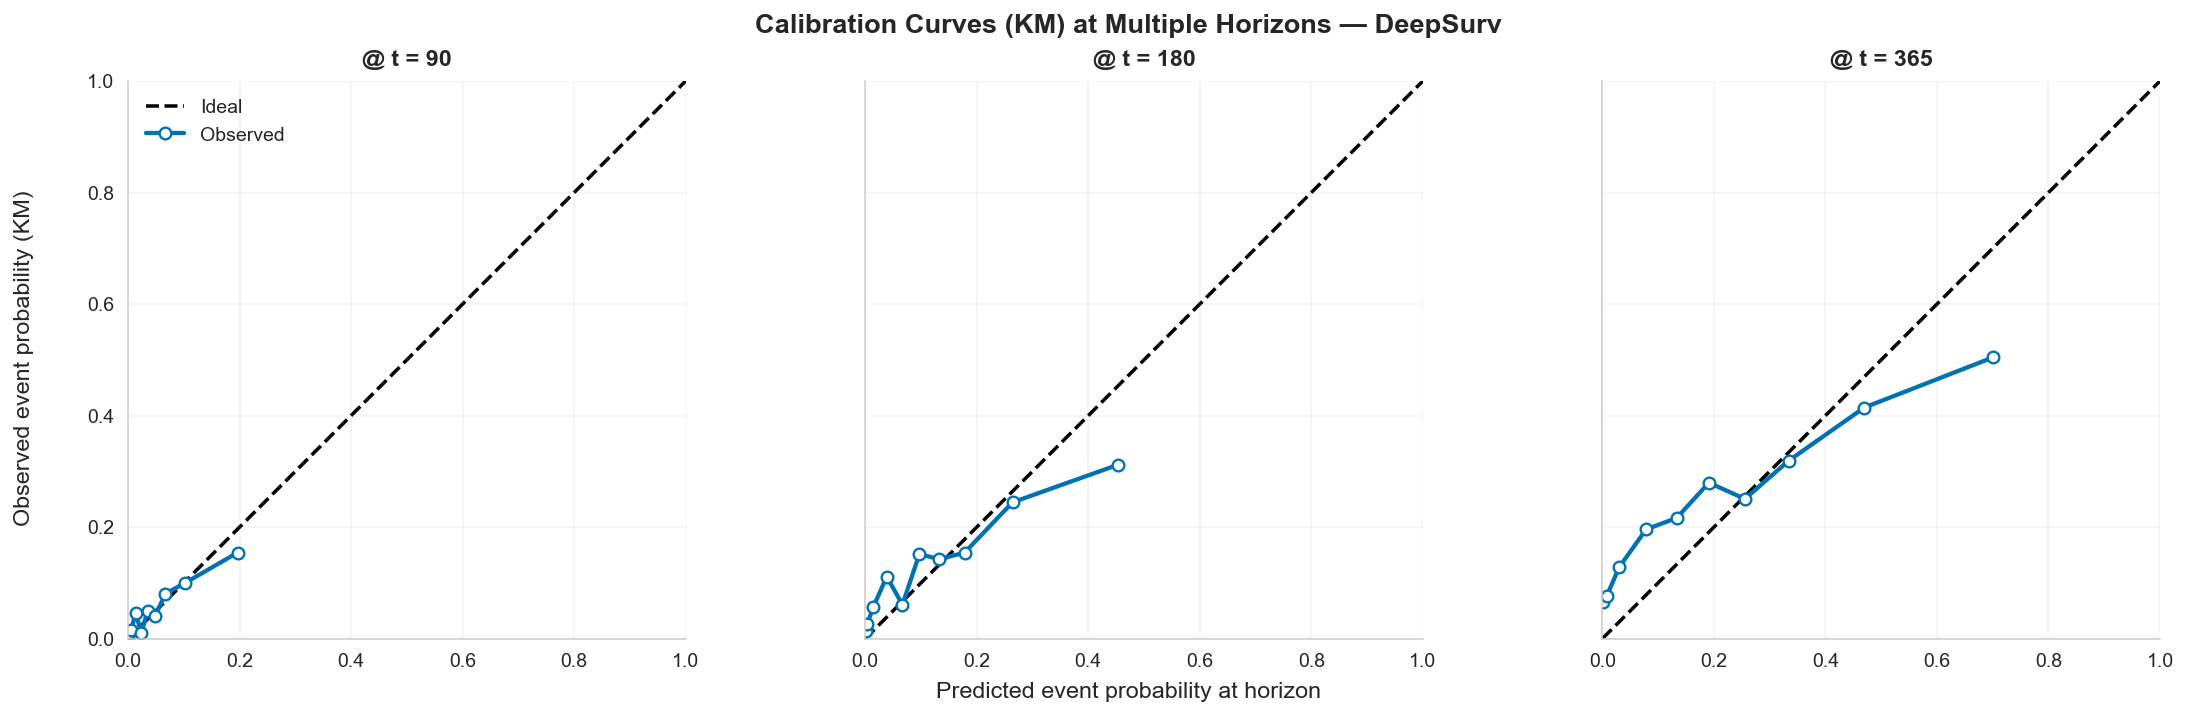
\includegraphics[width=\textwidth]{survival_images/deepsurv_calibration.png}
    \caption{Calibration plots for the DeepSurv model at 90, 180, and 365 hours.}
    \label{fig:deepsurv_calibration}
\end{figure}

\begin{figure}[htb!]
    \centering
    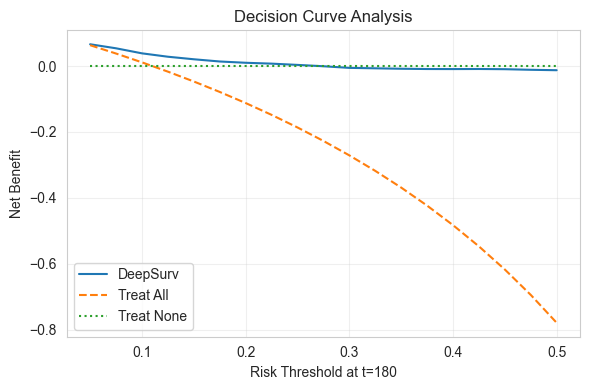
\includegraphics[width=0.7\textwidth]{survival_images/deepsurv_dca.png}
    \caption{Decision Curve Analysis for the DeepSurv model at a 180-hour horizon, demonstrating positive net benefit across a range of clinically relevant risk thresholds.}
    \label{fig:deepsurv_dca}
\end{figure}

\subsection{Synthesis of Survival Analysis}
Both the CoxPH and DeepSurv models delivered consistent and clinically interpretable predictions of time-to-death, with C-indices of 0.693 and 0.688, respectively. These results are comparable to those from other methodologically sound survival studies in critical care. For instance, \citet{Hu_2021} reported a C-index of 0.72 but used whole-stay aggregated features, which introduces a high risk of data leakage. The results obtained in the present work, derived strictly from T0--T24 data, therefore provide a more reliable and clinically actionable benchmark for early dynamic risk stratification in the SA--AKI population.

